\chapter{Autoregressive neural networks (ARNN)}
\label{sec:arnn}

In the previous chapter, we have seen the power of variational inference to approximate the free energy of intractable many-body systems. A crucial requirement for this method is a variational ansatz that supports efficient evaluation of normalized probability, and preferably has the rich expressiveness of neural networks. The search for this kind of variational ansatz has led to the development of autoregressive (AR) models, which have yielded the most prominent achievements in modern machine learning, and also find broad applications in many-body physics.

\section{Autoregressive factorization of joint probability}

We start from noticing that any joint probability $q(\vs)$ can be factorized into a product of conditional probabilities:
\begin{align}
q(\vs) &= \prod_i q_i(s_i \mid \vs_{< i}) \label{eq:autoreg} \\
&= q_1(s_1) q_2(s_2 \mid s_1) q_3(s_3 \mid s_1, s_2) \cdots q_N(s_N \mid s_1, s_2, \ldots, s_{N - 1}),
\end{align}
where we still assume that $\vs$ is a vector of $N$ spins, each can take the values $\pm 1$, and $\vs_{< i} = \{s_1, s_2, \ldots, s_{i - 1}\}$ denotes all variables before the $i$-th. This relation between random variables is called an AR model, which is a generalization from the traditional concept of AR in time series, where each random variable only have a linear dependency on the previous ones. In our case, the dependency can be arbitrarily nonlinear.

In principle, if the joint probability is known, one can compute the conditional probabilities by definition:
\begin{equation}
q_i(s_i \mid \vs_{< i}) = \frac{\sum_{\vs_{> i}} q(\vs)}{\sum_{\vs_{\ge i}} q(\vs)},
\end{equation}
which involves summations over exponentially many terms. However, neither do we know the joint probability in practice, nor can we exactly perform the summations. We generally parameterize the conditional probabilities by arbitrarily expressive neural networks, therefore the name ARNN, and use variational inference to optimize them towards the target distribution. The requirement of normalization in variational inference is particularly easy to fulfill under this factorization, because as long as each conditional probability is normalized: $\sum_{s_i} q_i(s_i \mid \vs_{< i}) = 1$, then the joint probability in \cref{eq:autoreg} will automatically be normalized. For binary variables, each conditional probability is naturally modeled by a Bernoulli distribution $\calB(s_i \mid \hat{s}_i) = (1 - \hat{s}_i) \delta_{s_i, -1} + \hat{s}_i \delta_{s_i, +1}$, which is always normalized and easy to sample from, and the parameter $\hat{s}_i$ can have an arbitrarily sophisticated dependency on the previous variables $\vs_{< i}$.

The joint probability of an AR model supports exact sampling, because we can sample the variables sequentially, following their order defined by the AR model. We first generate the value of $s_1$ from the independent distribution $q_1(s_1)$, then obtain the distribution $q_2(s_2 \mid s_1)$ and generate the value of $s_2$, then obtain the distribution $q_3(s_3 \mid s_1, s_2)$ and so forth, until all variables are generated. This procedure is also known as ancestral sampling. It involves $N$ sequential evaluations of the neural network, which can be a bottleneck in the time complexity of variational inference. On the other hand, when evaluating $q(\vs)$ given all variables $\vs$, all the conditional probabilities can be computed in parallel, which is comparatively not a concern in time complexity.

In the following, we introduce some neural network architectures to parameterize the conditional probabilities, each with its own use cases.

\begin{figure}[htb]
\centering
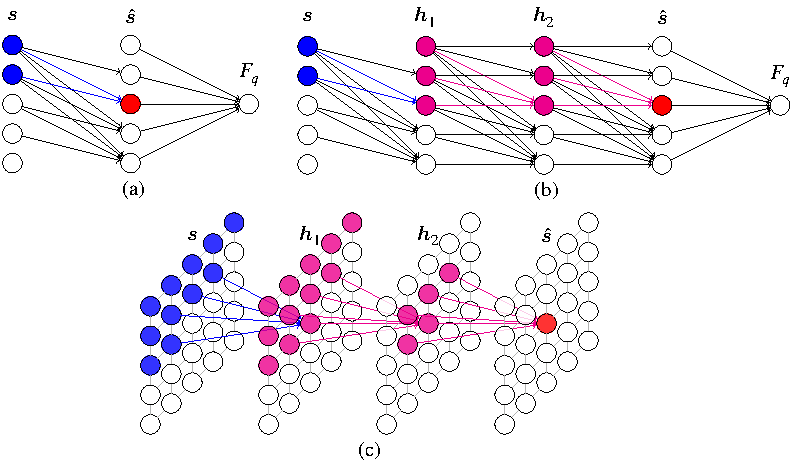
\includegraphics[width=0.9\linewidth]{ch5/arnn_arch.pdf}
\caption[Architectures of autoregressive neural networks (ARNN)]{
Architectures of dense and convolutional autoregressive neural networks (ARNN) for variational inference.
The spins $\vs$ are the inputs to the network.
The values $\hat{\vs}$ are the outputs from the network, which become parameters of the Bernoulli distributions.
The values $\vh_i$ are intermediate results in the network.
The variational free energy $F_q$ is given by \cref{eq:fq}, which depends on both the spins $\vs$ and the parameters $\hat{\vs}$.
The colored sites denote the receptive field of a site in $\hat{\vs}$, i.e., the input and the intermediate sites that an output site depends on.
(a) The network has only one layer, which is densely connected, and masked to ensure the AR property. The connections that are not masked out are illustrated as the arrows.
(b) The network has three masked dense layers.
(c) The network has three masked convolutional layers on a 2D lattice. In each layer, only the connections to one output site are shown for clarity, which depict the shape of the convolution kernel.
This figure is reproduced from Fig.~1 in Ref.~\cite{wu2019solving}.
}
\label{fig:arnn-arch}
\end{figure}

\section{Dense and convolutional ARNNs}

The most general way to parameterize the conditional probabilities is a dense feedforward neural network (FFNN) as in \cref{eq:ffnn}, which takes the spins $\vs$ as inputs, and outputs the parameters $\hat{\vs}$, then the conditional probabilities are modeled by the Bernoulli distributions $\calB(s_i \mid \hat{s}_i)$. The network needs to fulfill the AR property: each output $\hat{s}_i$ can only depend on the previous inputs $\vs_{< i}$. For a single dense layer, this is achieved by applying a triangular mask on the weight matrix in \cref{eq:linear-layer}:
\begin{gather}
\text{MaskedLin}(\vx) = (\mM \odot \mW) \vx + \mb, \\
M_{i j} = \begin{cases}
1, & i > j \\
0, & i \le j
\end{cases},
\end{gather}
where $\odot$ denotes the element-wise multiplication. This masked linear layer is illustrated in \cref{fig:arnn-arch}~(a). Multiple linear layers can be applied to improve the expressiveness of the network, and only one layer needs to mask out the connections $M_{i i}$, as shown in \cref{fig:arnn-arch}~(b). This architecture is known as masked autoencoder for distribution estimation (MADE)~\cite{germain2015made}.

Convolutional layers can also be applied to utilize the translational symmetry and the locality of the physical system, with the same mask $\mM$ to ensure the AR property. However, unlike a single convolutional FFNN, the joint probability $q(\vs)$ of a convolutional ARNN is not translational invariant as in \cref{eq:trans-invar}. The ARNN always assigns an artificial order of the spins to factorize the joint probability, thus breaks the translational symmetry. Instead, the purpose of convolutions in ARNN should be understood as enforcing the translational invariance of certain rules to determine the effect of the local environment on a spin.

An early application of 1D convolutional ARNN is the modeling of audios, known as WaveNet~\cite{oord2016wavenet}. The 2D convolutional ARNN has been similarly applied to the modeling of images, known as PixelCNN~\cite{oord2016pixel}, whose shape of the 2D convolutional kernel is illustrated in \cref{fig:arnn-arch}~(c). These ARNN architectures have also been introduced to the modeling of many-body systems, originally under the name of variational autoregressive networks (VAN)~\cite{wu2019solving}, and achieved superior results compared to traditional variational ansatzes.

Besides the dense and the convolutional ones, another widely used family of ARNNs is the recurrent neural networks (RNN), which incorporate the translational symmetry of the physical system in another way. They maintain the AR property by updating of some hidden variables $\vh^{(i)}$, also known as ``memories'', at each AR step $i$:
\begin{align}
\vh^{(i)} &= f\left( s_{i - 1}, \vh^{(i - 1)} \right), \\
\hat{s}_i &= g\left( \vh^{(i)} \right),
\end{align}
where $f$ and $g$ can be arbitrarily sophisticated neural networks, and their parameters are usually shared between sites. Because of the parameter sharing, RNNs can achieve satisfactory results with fewer parameters than dense networks. More variants of RNNs, including hybrids with CNNs and tensor networks, are also used in practice~\cite{oord2016pixel, khandoker2023supplementing}. Notably, the popular large language models in modern machine learning have essentially inherited the principles of RNN~\cite{brown2020language}.

\todo{Mention hierarchical and frequency-space ARNN}

\subsection{Numerical results}

\subsubsection{Square Ising model}

\begin{figure}[htb]
\centering
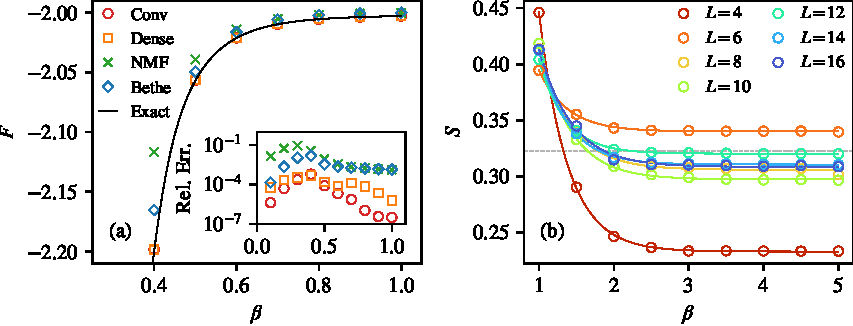
\includegraphics[width=\linewidth]{ch5/arnn_ising.pdf}
\caption[ARNN results of Ising model on square and triangular lattices]{
(a) Free energy per site of the ferromagnetic (FM) Ising model on the $16 \times 16$ square lattice with periodic boundary conditions (PBC), given by a dense ARNN and a convolutional ARNN, compared to the exact result~\cite{onsager1944crystal} and the traditional methods of naive mean field (NMF) and Bethe ansatz.
The inset shows the relative error of the variational result compared to the exact result. \\
(b) Entropy per site of the frustrated antiferromagnetic (AFM) Ising model on triangular lattices of various sizes $N = L \times L$ with PBC, given by a convolutional ARNN.
The curves are least-square fittings of $S / N = a \rme^{-b \beta} + c$, where $a, b, c$ are parameters for fitting, and $c$ is the residual  entropy when $\beta \to \infty$.
The horizontal dashed line indicates the exact result $S / N = \frac{2}{\pi} \int_0^{\frac{\pi}{3}} \ln(2 \cos \omega) \dd \omega \approx 0.323$ when $\beta \to \infty$ and $L \to \infty$~\cite{wannier1950antiferromagnetism, wannier1973antiferromagnetism}.
Note that the curves for $L = 8, 14, 16$ are almost overlapped.
This figure is reproduced from Fig.~2 in Ref.~\cite{wu2019solving}.
}
\label{fig:arnn-ising}
\end{figure}

We first demonstrate the performance of ARNN on the well-studied ferromagnetic (FM) Ising model on the $10 \times 10$ square lattice with periodic boundary conditions (PBC), where the analytical result~\cite{onsager1944crystal} and the traditional methods of naive mean field (NMF) ansatz in \cref{sec:nmf} and Bethe ansatz in \cref{sec:bethe} are available for comparison. A dense ARNN and a convolutional ARNN are trained on the Boltzmann distribution of this Hamiltonian, whose hyperparameters, such as the number of layers, the number of channels, and the convolution kernel size are selected to produce the lowest variational free energies within a reasonable computation budget. The networks are trained from scratch at each inverse temperature $\beta = 0.1, 0.2, \ldots, 1$. \Cref{fig:arnn-ising}~(a) shows the results of free energy, where we can clearly see that the ARNNs produce superior results compared to the traditional ansatzes, whose relative errors are lower by orders of magnitude.

In particular, the results from the convolutional ARNN are generally more accurate than those from the dense one with a similar number of parameters, thanks to the utilization of the translational symmetry and the locality of the physical system. This comparison justifies the use of convolutional layers in ARNN, even though the overall joint probability is not translational invariant. However, this advantage diminishes around the critical temperature $\beta_c = \frac{1}{2} \ln(1 + \sqrt{2}) \approx 0.44$, where the correlation length of the physical system diverges until bounded by the system size, as discussed in \cref{sec:iat}. The convolutional neural network can capture such long-range correlations only if the size of its receptive field is at least comparable to the correlation length.

\subsubsection{Triangular Ising model}

Then we apply the convolutional ARNN to the more complicated problem of antiferromagnetic (AFM) Ising model on the triangular lattice with PBC, which is geometrically frustrated. As discussed in \cref{sec:mode-collapse}, the frustration leads to exponentially many degenerate ground states. The entropy of this system at zero temperature is $S = \ln N_\text{GS}$, where $N_\text{GS}$ is the number of ground states. In the thermodynamic limit $N \to \infty$, we assume $N_\text{GS} = A \rme^{c N}$, where $A$ and $c$ are parameters to be determined. Therefore, we have $S / N = \frac{1}{N} \ln A + c$, which converges to $c$ as $N \to \infty$, and $c$ is known as the residual entropy~\cite{wannier1950antiferromagnetism, mambrini1999residual, vanderstraeten2018residual}. The existence of a non-zero residual entropy indicates the exponentially large number of degenerate ground states, which poses challenge for MCMC methods and previous variational ansatzes to accurately count it, or merely count its order of magnitude. For the relatively simple case of triangular Ising model, the analytical result of the residual entropy has been derived~\cite{wannier1950antiferromagnetism, wannier1973antiferromagnetism}.

In \cref{fig:arnn-ising}~(b), the ARNN produces entropies that exponentially decay to a constant as $\beta \to \infty$ for each system size $L$, and converge to the analytical result as $L \to \infty$. This demonstrates the rich expressiveness of ARNN, which has the potential to accurately approximate exponentially complex target distributions using polynomial computation time and number of parameters.

\subsubsection{Hopfield model}

\begin{figure}[htb]
\centering
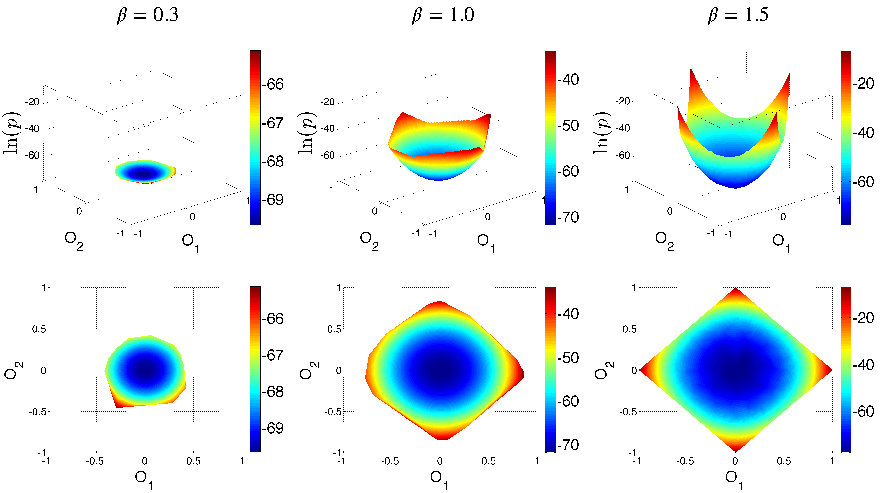
\includegraphics[width=\linewidth]{ch5/arnn_hop.pdf}
\caption[ARNN results of Hopfield model]{
Log-probability of samples from a dense ARNN, for the Hopfield model with $N = 100$ spins and $n_\text{p} = 2$ orthogonal patterns.
The top row shows the 3D view of the log-probability surfaces, and the bottom row shows the same results in the 2D view from top.
The columns are results with different inverse temperatures $\beta = 0.3, 1.0, 1.5$.
The $O_1$ and $O_2$ axes denote the overlaps between each sample and the two patterns respectively, as defined in \cref{eq:cl-overlap}.
The four ground states have $(O_1, O_2)$ = $(+1, 0)$, $(-1, 0)$, $(0, +1)$, $(0, -1)$ respectively.
This figure is reproduced from Fig.~3 in Ref.~\cite{wu2019solving}.
}
\label{fig:arnn-hop}
\end{figure}

An experiment to qualitatively study the ability of ARNN to capture multiple ground states is on the Hopfield model in \cref{eq:hopfield}. We construct a Hopfield model with $N = 100$ spins and $n_\text{p} = 2$ random orthogonal patterns, and train a dense ARNN that only consists of a single layer. Then we generate $10^4$ samples from the ARNN, and compute their probabilities and their overlaps with the two patterns respectively. \Cref{fig:arnn-hop} shows that the ARNN successfully samples the memorized patterns with exponentially higher probabilities than other states, in the retrieval phase with high $\beta$. This indicates the capability of ARNN to avoid mode collapse and capture all the modes separated by exponentially high energy barriers in this Hamiltonian.

\subsubsection{SK model}

\begin{figure}[htb]
\centering
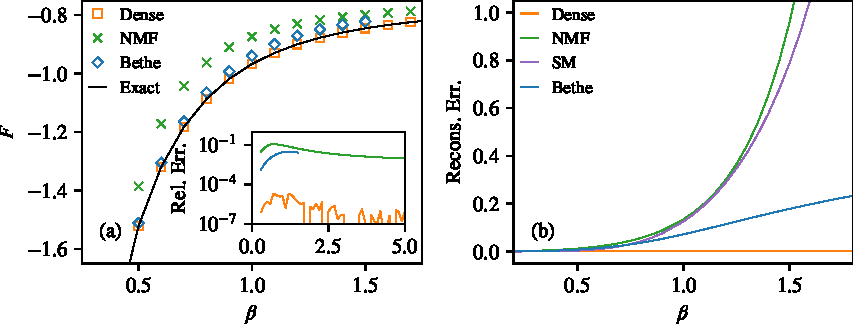
\includegraphics[width=\linewidth]{ch5/arnn_sk.pdf}
\caption[ARNN results of Sherrington--Kirkpatrick (SK) model and inverse SK problem]{
(a) Free energy per site for a random instance of the Sherrington--Kirkpatrick (SK) model with $N = 20$ spins, given by a dense ARNN, compared to the exact result by enumeration, the NMF ansatz, and the Bethe ansatz. The inset shows the relative error of the variational result compared to the exact result.
The iterative solution of the Bethe ansatz converges only when $\beta \le 1.5$. \\
(b) Reconstruction error of the inverse SK problem with $N = 20$ spins, given by a dense ARNN, compared to the NMF ansatz~\cite{roudi2009ising}, the Sessak--Monasson (SM) expansion~\cite{sessak2009small}, and the Bethe ansatz~\cite{ricci2012bethe}.
This figure is reproduced from Fig.~4 in Ref.~\cite{wu2019solving}.
}
\label{fig:arnn-sk}
\end{figure}

We also have the experiment on the Sherrington--Kirkpatrick (SK) model in \cref{sec:sk}, which has frustrated interactions with even higher complexity than the previous models. As a proof of concept, we generate a random instance of the SK model with $N = 20$ spins, and compute its properties by exact enumeration. Then we train a dense ARNN with a single layer. \Cref{fig:arnn-sk}~(a) shows that the ARNN still produces significantly more accurate approximation than traditional ansatzes for this Hamiltonian, especially in the glassy phase with high $\beta$ where the iterative solution of the Bethe ansatz fails to converge.

\subsubsection{Inverse SK problem}

Besides the ordinary problem of estimating the observables given the Hamiltonian, ARNNs can also be employed in the inverse SK problem, where we estimate the unknown interactions $\{J^*_{i j}\}$ given the correlations $\{C^*_{i j}\}$. Because each estimated correlation $\bbE_\text{MC}[C_{i j}]$ as in \cref{eq:monte-carlo} is a differentiable function of $\{J_{i j}\}$, we can directly use stochastic gradient descent to minimize the least-square loss
\begin{equation}
L\left( \{J_{i j}\} \right) = \frac{1}{N^2} \sum_{i j} \left( \bbE_\text{MC}[C_{i j}] - C^*_{i j} \right)^2.
\end{equation}
In this problem, we use an ARNN with two dense layers to estimate $C_{i j}$. The abilities of different methods to estimate the interactions is assessed by the reconstruction error
\begin{equation}
\text{Recons. Err.} = \frac{1}{N^2} \sum_{i j} \left( J_{i j} - J^*_{i j} \right)^2,
\end{equation}
where $J_{i j}$ are the estimated values and $J^*_{i j}$ are the true values. The results are shown in \cref{fig:arnn-ising}~(b), where the ARNN again outperforms traditional methods by a large margin.

\subsubsection{Remarks on network sizes}

It is worth discussing the sizes of the ARNNs used in the above experiments. For the fully connected cases of the Hopfield model, the SK model, and the inverse SK problem, we use small ARNNs containing only $O(N^2)$ parameters, and they produce significantly better results than the Bethe ansatzes with the same order of parameters. For the Ising models on the $16 \times 16$ square and triangular lattices, however, the ARNNs with the optimal variational free energies we have found contain as many as $O(10^6)$ parameters, while the Bethe ansatzes only contain $O(10^3)$. The large number of parameters also leads to significantly more computation time to evaluate the observables, as the training and the sampling of such a large neural network typically take several hours on a modern GPU, while the NMF ansatz and the Bethe ansatz can be solved almost instantly. Therefore, many use cases of neural networks to replace traditional ansatzes appear only in the regime where we seek much higher accuracy at the cost of correspondingly more computation. The comparison of neural networks and traditional methods under the same computation budget will be discussed in \cref{sec:arnn-mcmc}.

Apart from training a new network with each system size and temperature, it has also been proposed to directly reuse or fine-tune a trained network with different system sizes and temperatures~\cite{efthymiou2019super, mills2019extensive, rende2024fine}. This line of research opens a promising way to numerically compute the renormalization group (RG) flow, and extrapolate the critical temperature to the thermodynamic limit~\cite{ron2002inverse}.

\section{Sparse two-body ARNN}



This architecture is named TwoBo, because the authors were tired of the ever-growing lengths of acronyms.



\cite{pan2021solving}

\cite{biazzo2023autoregressive}

\cite{biazzo2024sparse}


\begin{figure}[htb]
\centering
\hspace*{\fill}
\subfloat[]{\raisebox{0.055\linewidth}{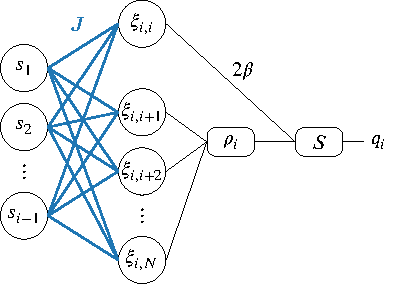
\includegraphics[width=0.4\linewidth]{ch5/twobo_arch.pdf}}}
\hspace*{\fill}
\subfloat[]{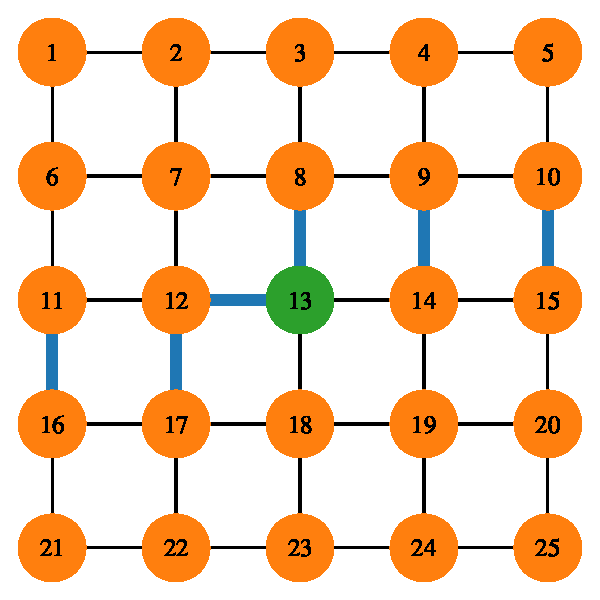
\includegraphics[width=0.4\linewidth]{ch5/twobo_grid_2d.pdf}}
\hspace*{\fill}
\caption{
(a) Sketch of the TwoBo ARNN architecture to compute a conditional probability $q_i(s_i = +1 \mid \vs_{< i})$.
The parameters of the first layer are directly taken from the interaction matrix $\bm{J}$.
The function $\rho_i$ is parameterized by a FFNN, whose inputs are the variables $\vxi_i$ after the first layer.
The last activation function $S$ is the sigmoid function in \cref{eq:sigmoid}. \\
(b) Calculating the conditional probability $q_i(s_i \mid \vs_{< i})$ with $i = 13$ on a 2D grid of $N = 25$ spins. The edges between the spins $\vs_{< i}$ and $\vs_{\ge i}$ are highlighted in blue, and only those edges are used when computing the intermediate variable $\xi_{i l}$. Therefore, among the variables $\{\xi_{i l} \mid l > i\}$, only those with $l < i + L$ are kept as inputs to $\rho_i$, and the others are ensured to be zero, which enhances the sparsity of the TwoBo network.
This figure is reproduced from Fig.~1 in Ref.~\cite{biazzo2024sparse}.
}
\label{fig:twobo-arch-grid}
\end{figure}

\subsection{Numerical results}

\subsubsection{Variational free energy}

\begin{figure}[htb]
\centering
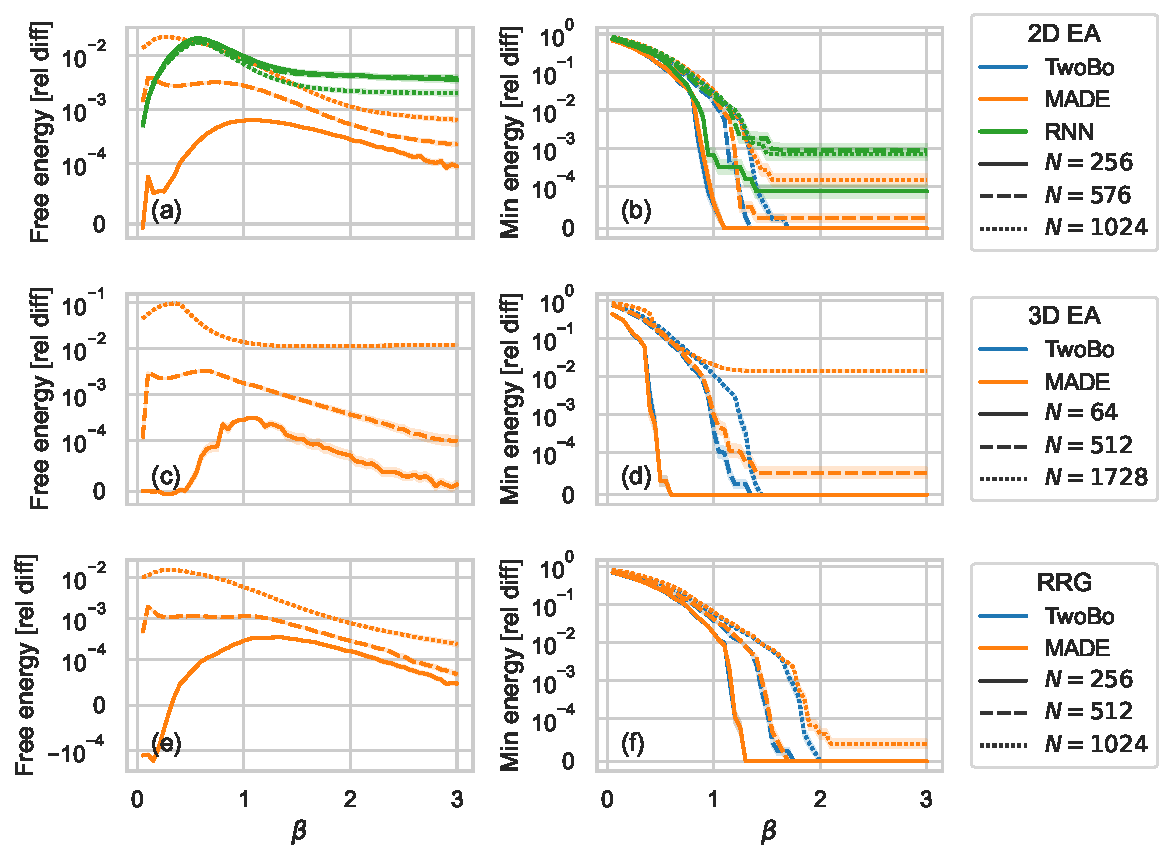
\includegraphics[width=\linewidth]{ch5/twobo_ea_rrg.pdf}
\caption{
Variational free energy (left column) and minimum energy of sampled configurations (right column) at each $\beta$ on 2D EA (top row), 3D EA (middle row), and RRG (bottom row) models of different sizes. We compare the performances of TwoBo, MADE, and RNN (only in 2D).
The variational free energy is shown as the relative difference from TwoBo at the same $\beta$, and the minimum energy as the relative difference from the one found by TwoBo at $\beta = 3$.
The results are averaged over $10$ random instances of the Hamiltonian, and the error bars show the standard errors over the instances.
This figure is reproduced from Fig.~2 in Ref.~\cite{biazzo2024sparse}.
}
\label{fig:twobo-ea-rrg}
\end{figure}

\subsubsection{Convergence of training}

\begin{figure}[htb]
\centering
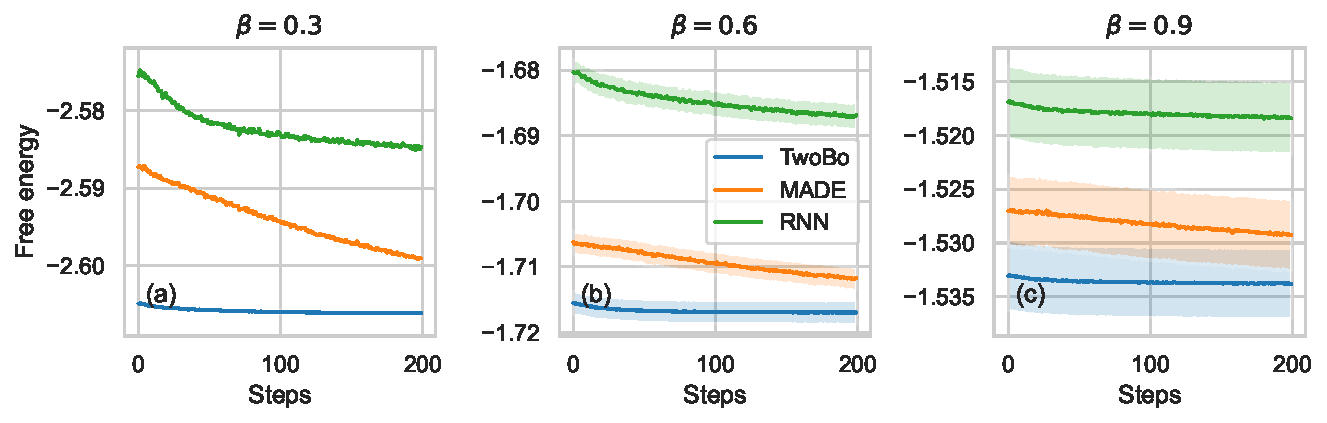
\includegraphics[width=\linewidth]{ch5/twobo_converge.pdf}
\caption{
Convergence of variational free energy when training at fixed values of $\beta$ on 2D EA model with $N = 14^2 = 576$.
The results are averaged over $10$ random instances of the Hamiltonian, and the error bars show the standard errors over the instances.
This figure is reproduced from Fig.~3 in Ref.~\cite{biazzo2024sparse}.
}
\label{fig:twobo-converge}
\end{figure}

\begin{figure}[htb]
\centering
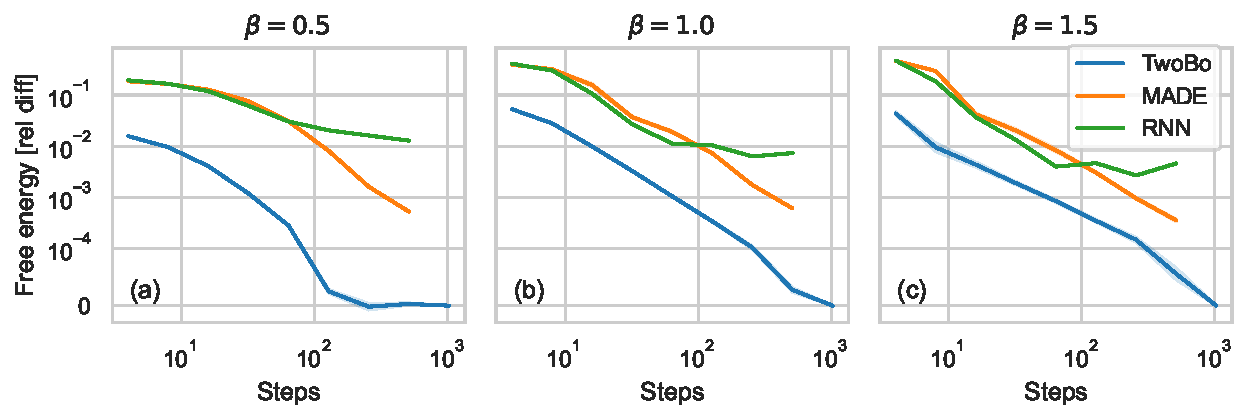
\includegraphics[width=\linewidth]{ch5/twobo_converge_max_steps.pdf}
\caption{
Variational free energy using different numbers of optimization steps at each $\beta$ on 2D EA model with $N = 576$, shown as the relative difference from TwoBo at the same $\beta$ using 1024 steps.
The results are averaged over $10$ random instances of the Hamiltonian, and the standard errors over the instances are too small to be visible.
This figure is reproduced from Fig.~4 in Ref.~\cite{biazzo2024sparse}.
}
\label{fig:twobo-converge-max-steps}
\end{figure}

\subsubsection{Parameter efficiency}

\begin{figure}[htb]
\centering
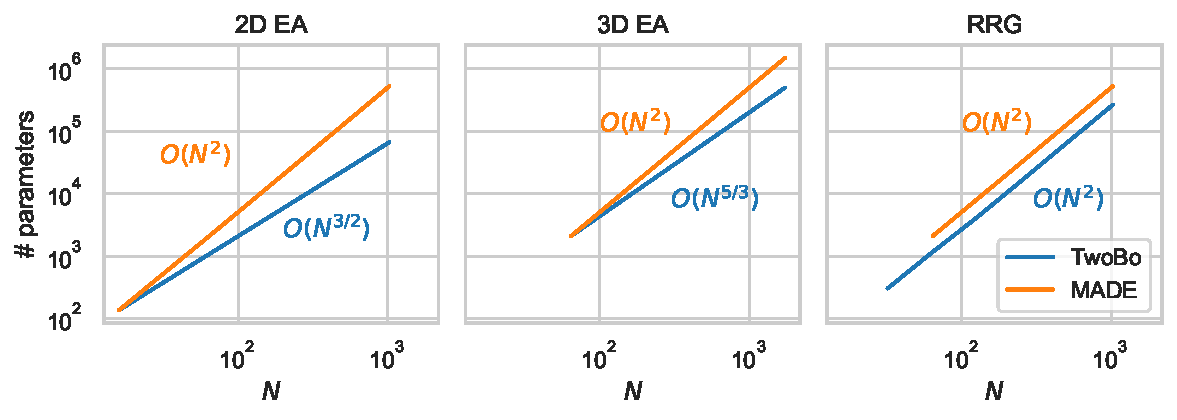
\includegraphics[width=\linewidth]{ch5/twobo_param.pdf}
\caption{
Number of trainable parameters in TwoBo and MADE on 2D EA, 3D EA, and RRG models of various system sizes $N$.
For RRG, the number of trainable parameters in TwoBo is averaged over $10$ random instances.
This figure is reproduced from Fig.~S1 in the supplementary material of Ref.~\cite{biazzo2024sparse}.
}
\label{fig:twobo-param}
\end{figure}

\begin{figure}[htb]
\centering
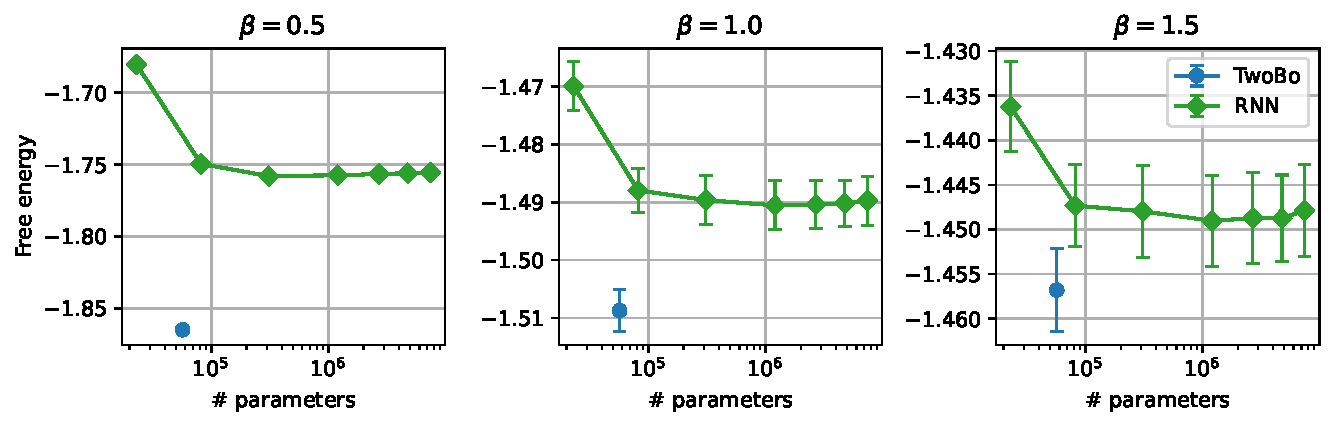
\includegraphics[width=\linewidth]{ch5/twobo_rnn_param.pdf}
\caption{
Variational free energy of TwoBo compared to RNN with different numbers of memory units ($2, 4, 8, 16, 24, 32, 40$), on 2D EA model with $N = 576$.
The results are averaged over $10$ random instances of the Hamiltonian, and the error bars show the standard errors over the instances.
This figure is reproduced from Fig.~S3 in the supplementary material of Ref.~\cite{biazzo2024sparse}.
}
\label{fig:compare_rnn}
\end{figure}

\section{ARNN in MCMC importance sampling}
\label{sec:arnn-mcmc}

\cite{nicoli2020asymptotically}

\cite{ciarella2023machine}

\subsection{Neural cluster updates}
\label{sec:ncus}

\cite{wu2021unbiased}

\subsection{Numerical results}
